%!TEX root = thesis.tex
%%%%%%%%%%%%%%%%%%%%%
%%%%%%%%%%%%%%%%%%%%%%%%%%%%%%%%%%%%%%%%%%%%%%%%%%
%%%%%%%%%%%%%%%%%%%%%%%%%%%%%%%%%%%%%%%%%%%%%%%%%%
\chapter{On the quantization of motion and fields}
\label{ch:on_quantization}
%%%%%%%%%%%%%%%%%%%%%%%%%%%%%%%%%%%%%%%%%%%%%%%%%%
%%%%%%%%%%%%%%%%%%%%%%%%%%%%%%%%%%%%%%%%%%%%%%%%%%
%
%
% In the introductory sections I am being pragmatic on purpose, in a sense of trading mathematical rigor with a comprehensive introduction in the theory concepts to safely guide the reader through the computations performed later in this thesis.\\
As an undergraduate student studying elementary physics, I always thought of quantum particles as plain waves living in the differential-geometric world of ``first quan\-ti\-zation'' which (at least for me) is both beautiful and frustrating at the same time as the task of solving the most simple problems may become quite involved, if not even impossible.
The modern approach is not a straightforward attempt to solve the real-space wave function by integrating a given Schrödinger equation, it rather sticks to an alternative representation in the algebraic world of ``second quantization'' where the action of operators dictate all physical consequences.
I must admit that I find the nomenclature of ``first'' and ``second'' somewhat confusing, as there is no such thing as two consecutive ways of quantization -- it's just two alternative and consistent ways of describing the same theory.
Ultimately, I've learned to accept this issue as a result of chronology: the original formulation of quantum mechanics is commonly called first quantization, in which the (motion of the) particle is quantized and possible electromagnetic fields or potentials are considered classical, wheres quantized fields have been formulated in the language of second quantization.
However, as we will see soon, the advantage of second quantization manifests itself in a simpler and more efficient way to describe many-body systems such that its development can be seen as the first major cornerstone in the development of quantum field theory.
\\

Regardless on the formulation, be it first or second, all quantum theories require certain basic concepts:
all quantum states are represented by state vectors $\{|q\rangle\}$ forming a complete basis of the Hilbert space and observables are defined through Hermitian operators acting on that space.
The states are given through a set of good quantum numbers $q$, e.g. $(n,l,m)$ associated to the total energy, angular momentum and its projection along the primary axis for the electron of hydrogen.
The first section ``On the quantization of motion and fields'' reviews these basic concepts in more detail and outlines the solution of atoms trapped in a harmonic potential in both differential and algebraic formulation.
I will also illustrate the treatment of small perturbations on top of a quadratic/non-interacting Hamiltonian which is a crucial tool in the understanding of quantum matter.
The importance of these solutions becomes clear after I introduce Luttinger liquids as first example of a quantum field theory satisfying the algebra of a quantum harmonic oscillator.
\\

Ultimately, there is few detailed things to say analytically about truly many-body phases of matter as the complexity of finding a full solution scales exponentially with the number of constituents.
This stresses the need of numerical techniques in the study of non-perturbative regimes which cannot be amended analytically.
In this thesis, I mainly use matrix product states, which is why I provide a section here which highlights the basic ideas and outlines benefits and shortcomings compared to other techniques.

Perhaps the most interesting behavior of quantum many-body physics is that of so-called emergent phenomena -- e.g. the appearance of quasi-particles which extend the canonical statistical properties of fermions and bosons in low dimensions, or the presence of robust quasi-particles at the boundaries of a topological insulator.
In order to perceive a basic overview in this topic, I conclude the introduction with a review on the classification of non-interacting topological matter and finish with some general statements on interacting topological insulators.
\\

The present chapter is inspired by a number of excellent books and lectures such as~\cite{AltlandSimons2010,BruusFlensberg2004,FetterWalecka2003} extending the basic aspects of quantum mechanics to a modern way of understanding quantum field theory in general.

%%%%%%%%%%%%%%%%%%%%%%%%%%%%%%%%%%%%%%%%%%%%%%%%
\section{Creation and annihilation operators}
\label{sec:creation_and_annihilation_operators}
%%%%%%%%%%%%%%%%%%%%%%%%%%%%%%%%%%%%%%%%%%%%%%%%
Consider a complete set of quantum numbers $\{\alpha\}$ which label a normalized set of states $\{\ket{\alpha}\}$ spanning the full Hilbert space $\HS^1$ of a generic single particle system described by the (time-independent) Schrödinger equation
\begin{align}
    \MH \ket{\alpha} = \varepsilon_\alpha\ket{\alpha}.
\end{align}
The single particle wave function $\Psi_\alpha(r)$ of a quantum state occupying $\alpha$ is defined as the inner product of the vector $\ket{\alpha}$ with the real-space covector $\bra{r}\in\HS^*$, i.e.
\begin{align}
    \Psi_\alpha(r) \coloneqq \braket{r|\alpha}.
\end{align}
It is is thus understood as the coefficients for the basis transform $\ket{\alpha}\rightarrow\ket{r}$, i.e.
\begin{align}
    \ket{\alpha} = \int{\rm d}{r}\, \Psi_\alpha(r) \ket{r}.
\end{align}
According to the basic postulate of quantum mechanics, the two-particle wave function with quantum numbers $\alpha_1$ and $\alpha_2$ is given by the (anti-) symmetrized product
\begin{align}
    \Psi_{\alpha_1,\alpha_2,\nu}(r_1,r_2) = \frac1{\sqrt2}\left(\braket{r_1|\alpha_1}\braket{r_2|\alpha_2} + \nu\braket{r_2|\alpha_1}\braket{r_1|\alpha_2}\right),
\end{align}
depending on the particle statistics upon exchange of their position, i.e. $\nu=\pm1$ for bosons and fermions, respectively.
The two-particle wave function can thus be represented by a more simple inner product
\begin{align}
    \Psi_{\alpha_1,\alpha_2,\nu}(r_1,r_2) = \left(\bra{r_1}\otimes\bra{r_2}\right)\ket{\alpha_1 \alpha_2}_\nu
\end{align}
which is given by the symmetric Kronecker product
\begin{align}
    \ket{\alpha_1 \alpha_2}_\nu = \frac1{\sqrt2}\left(\ket{\alpha_1}\otimes\ket{\alpha_2} + \nu\ket{\alpha_2}\otimes\ket{\alpha_1}\right).
\end{align}
In general, the symmetric $N$-particle state vector is an element of the $N$-particle Hilbert space $\HS^N = \bigotimes_{i=1}^N\HS$ and reads
\begin{align}
    \ket{\alpha_1,\alpha_2,\dots,\alpha_N}_\nu = \frac1{\sqrt{N!\prod_{\alpha}(n_\alpha!)}}\sum_P \nu^{1-\sign{P}/2}\ket{\alpha_{P(1)}}\otimes\ket{\alpha_{P(2)}}\otimes\dots\otimes\ket{\alpha_{P(N)}}.
    \label{eq:symmetric_many_body_state}
\end{align}
In the above equation, we assume ordered quantum numbers (e.g. increasing positions along a wire, or increasing energies), denote the total number of particles with quantum number $\alpha$ as $n_\alpha$ and $\sign{P}$ the sign of the permutation $P\in S^N$ of the permutation group [$\sign{P}=\pm1$ if the permutation is even/odd].
\\

The representation in the ordered expression of \cref{eq:symmetric_many_body_state} is not particularly compact since equal values of $\alpha$ may appear $n_\alpha$ times in the $N$-letter long ket -- the occupation number representation removes this redundancy.
The states in this representation are then given by
\begin{align}
    \ket{n_1, n_2, \dots}_\nu = \ket{\underbrace{\alpha_1,\alpha_1,\dots,\alpha_1}_{n_1}, \underbrace{\alpha_2, \alpha_2,\dots, \alpha_2}_{n_2}, \alpha_3, \dots}
\end{align}
and they span the space $\FS^N$ of the symmetrized $N$-particle states $\sum_{i} n_i = N$.
Thus, the subset $\FS^N\subset \HS^N$ contains all $N$-particle states which transform according to the basic postulate of quantum mechanics such that any physical state $\ket{\Psi}\in\HS^N$ can be written as a linear superposition of the Fock states
\begin{align}
    \ket{\Psi}_\nu = \sum_{\sum_i n_i = N}c_{n_1,n_2,\dots}\ket{n_1,n_2,\dots}_\nu.
\end{align}
The full Fock space $\FS$ is defined as a direct sum of all vector spaces with fixed quantum number $N$, i.e.
\begin{align}
    \FS = \bigoplus_{N=0}^\infty \FS^N
\end{align}
including the one-dimensional vacuum space commonly denoted by $\{\ket{0}\}=\FS^0$.
\\

Let us now impose a linear map $a^\dag_i:\FS\rightarrow\FS$ connecting the individual subsets through
\begin{align}
    a^\dag_i\ket{n_1,\dots,n_i,\dots}_\nu = \sqrt{n_i+1}\nu^{\sum_{j<i}n_j}\ket{n_1,\dots,n_i+1,\dots}_\nu
    \label{eq:creation}
\end{align}
in which fermionic states must be understood ${\rm mod}_2$ such that the Pauli exclusion principle is explicitly satisfied: $a^\dag{}^2\ket{0}=a^\dag\ket{1}={\rm mod}_2(1+1)\ket{{\rm mod}_2(1+1)} = 0\ket{0} = 0$.
Notice that through the linear map we can express the canonical basis of any subset $\FS^N\subset\FS$ as
\begin{align}
    \ket{n_1,n_2,\dots}_\nu = \prod_i\frac1{\sqrt{n_i!}}\left(a^\dag_i\right)^{n_i}\ket{0}_\nu,
    \label{eq:Fock_basis}
\end{align}
and as such have a tool which promotes the vacuum to any state of the full Fock space.
\begin{figure}
    \centering
    \subfigure[]{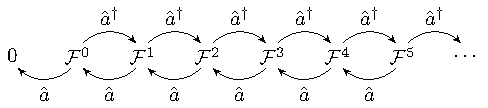
\includegraphics{figures/connected_fock_space_bosons.pdf}}
    \hfil
    \subfigure[]{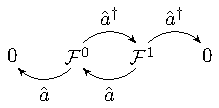
\includegraphics{figures/connected_fock_space_fermions.pdf}}
    \caption{(a) Subspaces $\FS^N$ of $N$-particle bosonic states $\ket{N}$ characterized by a single quantum number. Adjacent spaces are connected through the linear maps $a^{(\dag)}$ defined in \cref{eq:creation,eq:annihilation}. (b) Subspaces for a fermionic system characterized by a single quantum number.}
    \label{fig:my_label}
\end{figure}
Notice the absence of the phase $\nu$ on the right hand side which is due to the fact that the product is ordered.
For this reason, the linear maps $a^\dag_i$ are commonly called creation operators which is what we will call them in the remaining part of this thesis.
Two different linear maps $j<i$ satisfy the following equation
\begin{align}
    a^\dag_i a^\dag_j\ket{n_1,n_2,\dots}_\nu = \nu a^\dag_ja^\dag_i\ket{n_1,n_2,\dots}_\nu,
\end{align}
and thus span the famous (anti-) commutation relation
\begin{align}
    \commutator{a^\dag_i, a^\dag_j}_\nu \coloneqq a^\dag_i a^\dag_j - \nu a^\dag_j a^\dag_i = 0.
\end{align}
From the Hermitian adjoint of the equations before we get the condition
\begin{align}
   \braket{n_1,\dots,n_i,\dots | a^\pdag_i | m_1, \dots, m_i,\dots}_\nu =
   \sqrt{n_i+1}\nu^{\sum_{j<i}n_j} \delta_{n_1,m_1}\dots\delta_{n_i+1,m_i}\dots
\end{align}
and thus
\begin{align}
   a^\pdag_i \ket{n_1, \dots, n_i,\dots}_\nu =
   \sqrt{n_i}\nu^{\sum_{j<i}n_j} \ket{n_1, \dots, n_i-1,\dots}_\nu,
   \label{eq:annihilation}
\end{align}
from which we obtain the algebra relations of the creation/annihilation operators
\begin{align}
    \commutator{a^\pdag_i,a^\dag_j}_\nu = \delta_{i,j},
    \quad
    \commutator{a^\pdag_i,a^\pdag_j}_\nu = 0,
    \quad
    \commutator{a^\dag_i,a^\dag_j}_\nu = 0.
    \label{eq:Heisenberg_algebra}
\end{align}
Proceeding in a reversed manner,~\cref{eq:Fock_basis} is a consequence of the Stone-von Neumann theorem which states that, given the Heisenberg algebra defined through~\cref{eq:Heisenberg_algebra}, the action of the operators and the representation of the Fock basis is unique (up to unitary transformations)~\cite{Hall2013}.

To conclude this first section, a change of basis $\{\ket\alpha\}\rightarrow\{\ket\beta\}$ yields\footnote{Remember that $\mathbb1 = \sum_\alpha\ket{\alpha}\bra{\alpha}$, $\ket{\beta} = \sum_\alpha\ket{\alpha}\braket{\alpha|\beta}$ and $\ket{\beta}=a^\dag_\beta\ket{0}$, leading to \cref{eq:creation_annihilation_basis_rotation}.} a unitary transformation of the operators
\begin{align}
    a^\dag_\beta = \sum_\alpha \braket{\alpha|\beta}a^\dag_\alpha,
    \quad
    a^\pdag_\beta = \sum_\alpha \braket{\beta|\alpha}a^\pdag_\alpha
    \label{eq:creation_annihilation_basis_rotation}
\end{align}
which requires only a computation of the single-particle matrix elements $\braket{\alpha|\beta}$.
Before we move on to the representation of observables, a word on common notations: Quite often the authors assume a certain particle statistics and operator algebra at the beginning of their work which implies a constant (and thus dropped) subscript $\nu$.
In such cases, fermionic annihilation operators are mostly identified through the letter $c$ whereas $b$ often corresponds to bosonic operators.
Furthermore, a common convention identifies the commutator through crotchets
\begin{align}
    \left[\hat A,\hat B\right]\coloneqq\commutator{\hat A,\hat B}_+ = \hat A\hat B - \hat B\hat A
\end{align}
and the anticommutator through curly braces
\begin{align}
    \anticommutator{\hat A,\hat B}\coloneqq\commutator{\hat A,\hat B}_- = \hat A\hat B + \hat B\hat A.
\end{align}
Let me also provide a useful expression to evaluate the commutation relation of operator products recursively
\begin{align}
    \commutator{\hat A, \hat B \hat C}_\pm
    &= \hat A\hat B\hat C \mp \hat B\hat C\hat A + \hat B\hat A\hat C - \hat B\hat A\hat C
    \\
    &= \commutator{\hat A, \hat B}_\pm\hat C \mp \hat B\hat C\hat A \mp \hat B\hat A\hat C
    = \commutator{\hat A, \hat B}_\pm\hat C \mp \hat B\commutator{\hat A,\hat C}.
    \label{eq:recursive_commutation}
\end{align}
In many cases, the sets of quantum numbers are continuous (e.g. position $x$) and as such a sum in \cref{eq:creation_annihilation_basis_rotation} is promoted to an integral expression:
\begin{align}
    a(x) = \sum_\alpha \braket{x | \alpha} a_\alpha,
    \quad
    a_\alpha = \int{\rd x} \braket{\alpha | x} a(x).
\end{align}
This is commonly highlighted through a bracket notation of the continuous quantum number.
%
%
%%%%%%%%%%%%%%%%%%%%%%%%%%%%%%%%%%%%%%%%%%%%%%%
\section{Representation of generic operators}
\label{sec:representation_of_generic_operators}
%%%%%%%%%%%%%%%%%%%%%%%%%%%%%%%%%%%%%%%%%%%%%%%
Let us start with a general operator acting on a single particle of the full $N$-particle state (usually dubbed one-body operator).
Familiar examples are for example the momentum or the position operator $\hat x_i$, $\hat p_i$ acting on the $i$th particle, or compositions of those like single particle potentials $V(\hat x_i)$.
It is thus not surprizing that the general expression of such operators can be given in terms of the particle creation and annihilation operators we introduced in \cref{sec:creation_and_annihilation_operators}.
\\

A one-body operator $\hat o$ diagonal in an arbitrary single-particle basis $\{\alpha\}$ ($\hat o = \sum_\alpha o_{\alpha}\ket{\alpha}\bra{\alpha}$) is trivially extended to the $N$-particle states written in the same basis
\begin{align}
    \hat O_1
    = \sum_{\alpha_i} o_{\alpha_i}a^\dag_{\alpha_i}a^\pdag_{\alpha_i}.
\end{align}
This is most easily understood: one-body operators act on only a single entity of the full set of particles, leaving the others untouched.
In the diagonal basis of $\hat O_1$, the action of $\hat n_{\alpha_i}\coloneqq a^\dag_{\alpha_i}a^\pdag_{\alpha_i}$ just counts the number of particles in the state $\alpha_i$, which is then multiplied with the expectation value of the single-particle operator.
In a more general basis, the one-body operator transforms according to \cref{eq:creation_annihilation_basis_rotation} resulting in
\begin{align}
    \hat O_1 = \sum_{\alpha, \beta}\braket{\alpha | \hat o | \beta} a^\dag_\alpha a^\pdag_\beta = \sum_{\alpha,\beta}o_{\alpha,\beta}a^\dag_\alpha a^\pdag_\beta
    \label{eq:one_body_operator}
\end{align}
It is now straightforward to introduce generic $2$-body operators $\hat O_2$
\begin{align}
    \hat O_2 = \sum_{\alpha,\beta,\gamma,\delta}O_{\alpha,\beta,\gamma,\delta}a^\dag_\alpha a^\dag_\beta a^\pdag_\gamma a^\pdag_\delta
\end{align}
in which the expectation value reads $O_{\alpha,\beta,\gamma,\delta}\coloneqq \braket{\alpha,\beta | \hat o | \gamma,\delta}$.
For example, a generic two-point interaction $\hat V\ket{r_1,\dots,r_N}=1/2\sum_{n\neq m}V(r_n,r_m)\ket{r_1,\dots,r_N}$ in continuous space takes the second quantized form
\begin{align}
    \hat V = \frac12\int{\rd^d r}\int{\rd^d r'}V({\bf r}-{\bf r'})a^\dag({\bf r})a^\dag({\bf r'})a^\pdag({\bf r'})a^\pdag({\bf r}).
    \label{eq:two_point_interaction}
\end{align}
The generalization to generic $M$-body operators is now straightforward
\begin{align}
    \hat O_M = \sum_{\alpha_1,\dots,\alpha_M}\sum_{\beta_1,\dots,\beta_M}O_{\alpha_1,\dots,\alpha_M,\beta_1,\dots,\beta_M}a^\dag_{\alpha_1}\dots a^\dag_{\alpha_M}a^\pdag_{\beta_1}\dots a^\pdag_{\beta_M}.
\end{align}
%
%
%%%%%%%%%%%%%%%%%%%%%%%%%%%%%%%%
\section{Periodic potentials}
\label{sec:periodic_potentials}
%%%%%%%%%%%%%%%%%%%%%%%%%%%%%%%%
To get acquainted with the concept of second quantization, it will be useful to consider such systems which are effectively characterized by a Hamiltonian composed of generic one-body operators of the form \cref{eq:one_body_operator}, and interactions which do not alter the excitation spectrum of the non-interacting system.
In particular, we consider the usual Hamiltonian of free particles
\begin{align}
    \hat H_0 = \sum_s\int\rd^d r\, a^\dag_s({\bf r})\brlr{\frac{\hat p^2}{2m}+V_{ae}({\bf r})}a_s^\pdag({\bf r})
\end{align}
and impose generic two-body interactions
\begin{align}
    \hat V_{ee} = \frac12\sum_{s,s'}\int\rd^dr\int\rd^dr'\,V_{ee}({\bf r}-{\bf r'})a^\dag_s({\bf r})a^\dag_{s'}({\bf r'})a^\pdag_{s'}({\bf r})a^\pdag_{s}({\bf r})
\end{align}
with operators $a^\pdag_s({\bf r})$ annihilating a particle with flavor $s$ at position $\bf r$.
The term $V_{ae}$ is a collection of $N_a$ local potentials
\begin{align}
    V_{ae}({\bf r}) = \sum_{i=1}^{N_a}V_{ae}({\bf R}_i - {\bf r})
\end{align}
and the value of $V_{ae}$ is determined by the relative distance from the position ${\bf R}_i$.
If the creation operators satisfy the anticommutator algebra in real space
\begin{align}
    \anticommutator{a^\pdag_s({\bf r}),a^\dag_{s'}({\bf r'})}=\delta_{s,s'}\delta({\bf r}-{\bf r'}),
\end{align}
the Hamiltonian defines a spinful fermionic system embedded in a crystal lattice (e.g. electrons of traditional solid state setups).
The bare (Bravais) lattice structure in $d$ dimensions is in general spanned by $d$ linearly independent (not necessary mutually perpendicular and normalized) vectors ${\bf x}_i$ and can thus be defined as the set
\begin{align}
    \mathcal{R} = \anticommutator{\sum_{i=1}^d n_i {\bf x}_i,\ n_i\in\mathds Z}.
\end{align}
Additional vectors $\{{\bf b}_i\}$ (sometimes called the basis) are used to define the position of the potential minima relative to the points of the Bravais lattice, such that every position in the primitive cell is given by ${\bf R}_j = \sum_i n_i {\bf x}_i + {\bf b}_j$ with integers $n_i\in\mathds Z$.
The beauty of this approach becomes visible as soon as we define the lattice translation operator
\begin{align}
    \hat T_{\bf n} : \psi_\alpha({\bf r}) \mapsto \psi_\alpha\brlr{{\bf r}+T_{\bf n}},\ T_{\bf n}\coloneqq\sum_i n_i {\bf x}_i={\bf n}\underline{\bf x}
\end{align}
which translates every function from one position to a distance parametrized through the $d$-dimensional vector ${\bf n}\in\mathds Z^d$ and the collection of all lattice vectors $\underline{\bf x}\coloneqq ({\bf x}_1,\dots,{\bf x}_d)^T$.
The local potential $V_{ae}({\bf r})$ is per definition invariant under lattice translations, and the two-body interaction $V_{ee}({\bf r}-{\bf r'})$ is clearly invariant under continuous translations, such that the full Hamiltonian $\hat H$ commutes with the translation operator and we can write the spectrum in eigenfunctions of $\hat T_n$.
The eigenfunctions of all translation operators $\hat T_n$ are called Bloch waves and have the following properties\footnote{Note here that a further restriction on the values of the reciprocal lattice vector ${\bf k}$ arise from imposing boundary conditions. E.g. Born-von Karman boundary conditions imply a periodicity after $L_j$ unit translations $\psi_\alpha({\bf r}+ L_j{\bf R}_j)=\psi_\alpha({\bf r})$, which confines the allowed values of $k_j$ to multiples of $\frac{\bf G_j}{L_j}$ in which $\bf G_j$ is the reciprocal vector of ${\bf R}_j$, i.e. ${\bf G}_j {\bf R}_j = 2\pi/a$.}
\begin{align}
    \hat T_{\bf n}\psi_{\alpha}({\bf r}) &= c_{\bf n}\psi_{\alpha}({\bf r})\\
    c_{{\bf n}_1}c_{{\bf n}_2} &= c_{{\bf n}_1+{\bf n}_2} \Rightarrow c_{\bf n} = \re^{{\bf s}{\bf n}\underline{\bf x}},\ {\bf s}\in\mathds C^d\\
    1=\int_V\rd^dr\,\abs{\psi_{\alpha}({\bf r})}^2 &= \int_V\rd^dr\,\abs{\hat T_{\bf n}\psi_{\alpha}({\bf r})}^2 \Rightarrow 1=\abs{c_{\bf n}}^2 \Rightarrow {\bf s}=\ri{\bf k},\ {\bf k}\in\mathds R^d
\end{align}
It is now possible to phrase Bloch's theorem, which states that the eigenfunctions of a particle moving in periodic potentials assume the simple structure
\begin{align}
    \psi_\alpha({\bf r}) = \psi_{\alpha{\bf k}}({\bf r}) = \re^{\ri{\bf k}{\bf r}}u_{\alpha{\bf k}}({\bf r}).
    \label{eq:bloch_theorem}
\end{align}
Note that we introduced the translation operators eigenvalue argument $\bf k$ in the list of good quantum numbers.
In particular, $\psi$ is a weighted plane wave in which $u$ inherits the lattice periodicity
\begin{align}
    \hat T_{\bf n} u_{\alpha{\bf k}}({\bf r})
    =
    \re^{-\ri{\bf k}\brlr{{\bf r}+{\bf n}\underline{\bf x}}}c_{\bf n}\psi_{\alpha{\bf k}}({\bf r})
    =
    \re^{-\ri{\bf k}{\bf r}}\re^{-\ri{\bf k}{\bf n}\underline{\bf x}}c_{\bf n}\psi_{\alpha{\bf k}}({\bf r})
    =
    u({\bf r}).
\end{align}
The particular expression of the weights obviously depends on the potential, and even for simple problems general solutions become quite involved\footnote{Except maybe the trivial scenario $V_{ae}({\bf r})={\rm const.}$ which implies to set $u=1$ in \cref{eq:bloch_theorem}.}.
In general, the wave vector $\bf k$ seems to play the same role as the particle momentum $\bf p$ in the Sommerfeld theory of a free particle.
However, this is not true as is clear from the momentum operator being $\hat{\bf p}=-\ri\hbar\nabla$, and as such
\begin{align}
  \hat{\bf p}\psi_{\alpha{\bf k}}({\bf r}) = \hbar{\bf k}\psi_{\alpha{\bf k}} - \ri\hbar\re^{\ri{\bf k}{\bf r}}\nabla u_{\bf k}(\bf r).
\end{align}
The vector ${\bf k}$ is thus dubbed crystal momentum, remembering the fact that $\psi_{\alpha{\bf k}}$ is only an eigenstate of momentum if the potential is a constant and $\nabla V_{ae}=0$.
Derivation of the effective potential $V_{ae}$ for real materials and analytic solutions of the Bloch weights $u$ are often quite involved and not of particular interest for this thesis (for more details, see~\cite{AshcroftMermin1978,Czycholl2016}).
Moreover, the introduction of tightly bound systems makes clear that a full knowledge of $u$ is not necessary to characterize the spectrum of such systems.
%
%
%%%%%%%%%%%%%%%%%%%%%%%%%%%%%%%%%%
\section{Tight binding systems}
\label{sec:tight_binding_systems}
%%%%%%%%%%%%%%%%%%%%%%%%%%%%%%%%%%
The systems considered here are those of tightly bound constituents to the lattice centers.
Such types can be found in traditional solid state scenarios where the nuclei are well separated beyond the typical Bohr radius of the valence electrons, in setups of ultracold atoms trapped in optical lattices (see \cref{ch:ultracold_atoms_trapped_in_optical_lattices}), in optical waveguides or polaritons.
In \cref{part:results}, I will mostly cover theoretical aspects of tight binding models which can be experimentally realized in a variety of different setups.
For this reason, it will be useful to review briefly how these models are motivated in general from a more traditional solid state aspect, and how they can be understood in the more modern approach of second quantization.
\\

For this purpose, we assume the problem of the single-particle Hamiltonian $\hat H_0$ to be fully solved, such that the Bloch states $\psi_{\alpha{\bf k}}$ are determined, diagonalize $\hat H_0$ and have energy eigenvalues $\varepsilon_{\alpha{\bf k}}$.
This allows to introduce the Wannier basis -- a localized basis composed of the Bloch states and defined as
\begin{align}
    \ket{w_{\alpha{\bf R}}} = \frac1{\sqrt N}\sum_{\bf k}\re^{-\ri{\bf k}{\bf R}}\ket{\psi_{\alpha{\bf k}}}.
    \label{eq:wannier_states}
\end{align}
We can translate this to the language of second quantization by the notion that
the transformation between Bloch and Wannier basis is unitary, such that annihilation and creation operators of Wannier and Bloch states are set in relation by
\begin{align}
    a^\dag_{\alpha{\bf R}s} = \frac1{\sqrt N}\sum_{\bf k}\re^{-\ri{\bf k}{\bf R}}a^\dag_{\alpha{\bf k}s},
    \quad
    a^\dag_{\alpha{\bf k}s} = \frac1{\sqrt N}\sum_{\bf R}\re^{+\ri{\bf k}{\bf R}}a^\dag_{\alpha{\bf R}s}.
    \label{eq:wannier_states_2}
\end{align}
Now, the free Hamiltonian is diagonal in the Bloch basis with energies $\varepsilon_{\alpha{\bf k}} = \int\rd^dr\, \psi_{\alpha{\bf k}}^* \hat H_0 \psi_{\alpha{\bf k}}$ and can be rewritten as
\begin{align}
    \hat H_0
    =
    \sum_{{\bf k},s}\varepsilon_{\alpha{\bf k}}a^\dag_{\alpha{\bf k}s}a^\pdag_{\alpha{\bf k}s}
    \overset{\text{\cref{eq:wannier_states_2}}}{=}
    \frac1N\sum_{\bf R, R', k}
    \re^{\ri{\bf k}\brlr{{\bf R}-{\bf R'}}}
    \varepsilon_{\alpha{\bf k}}
    a^\dag_{\alpha{\bf R}s}a^\pdag_{\alpha{\bf R'}s}
    =
    \sum_{i, j}t_{\alpha,i,j}
    a^\dag_{\alpha{\bf R}_is}a^\pdag_{\alpha{\bf R}_js}
    \label{eq:tight_binding_hamiltonian}
\end{align}
in which the matrix element $t_{\alpha,i,j}$ denotes the strength of the scattering process between two lattice centers, to be determined through the energy bands
\begin{align}
    t_{\alpha,i,j} \coloneqq \frac1N\sum_{\bf k}\re^{\ri{\bf k}\brlr{{\bf R}_i-{\bf R}_j}}\varepsilon_{\alpha{\bf k}}.
\end{align}
On a more abstract level, the Hamiltonian \cref{eq:tight_binding_hamiltonian} denotes quantum particles hopping between lattice sites which are connected through the matrix $t_{\alpha}$.
Similarly, the interaction $\hat V_{ee}$ can be written as
\begin{align}
    \hat V_{ee} = \sum_{i,i',j,j'}\sum_{\beta,s,s'}U_{i,i',j,j'}a^\dag_{\alpha,{\bf R}_is}a^\dag_{\beta,{\bf R}_{i'}s'}a^\pdag_{\beta,{\bf R}_js'}a^\pdag_{\alpha,{\bf R}_{j'}s}
\end{align}
%
%
%%%%%%%%%%%%%%%%%%%%%%%%%%%%%%
\section{Luttinger liquids}
\label{sec:luttinger_liquids}
%%%%%%%%%%%%%%%%%%%%%%%%%%%%%%
We are interested to build an effective model in one dimension capturing the relevant degrees of freedom at low temperatures.
With that purpose, let us start by the free fermionic 1D Hamiltonian $\hat H_0$ denoted by the following (diagonal) representation in momentum space
\begin{align}
    \hat H_0 = \sum_k \frac{k^2}{2m}\hat n_k
\end{align}
with dispersion relation $\varepsilon_k =\frac{k^2}{2m}$ depicted in \cref{fig:1D_quadratic_dispersion}.
\begin{figure}
    \centering
    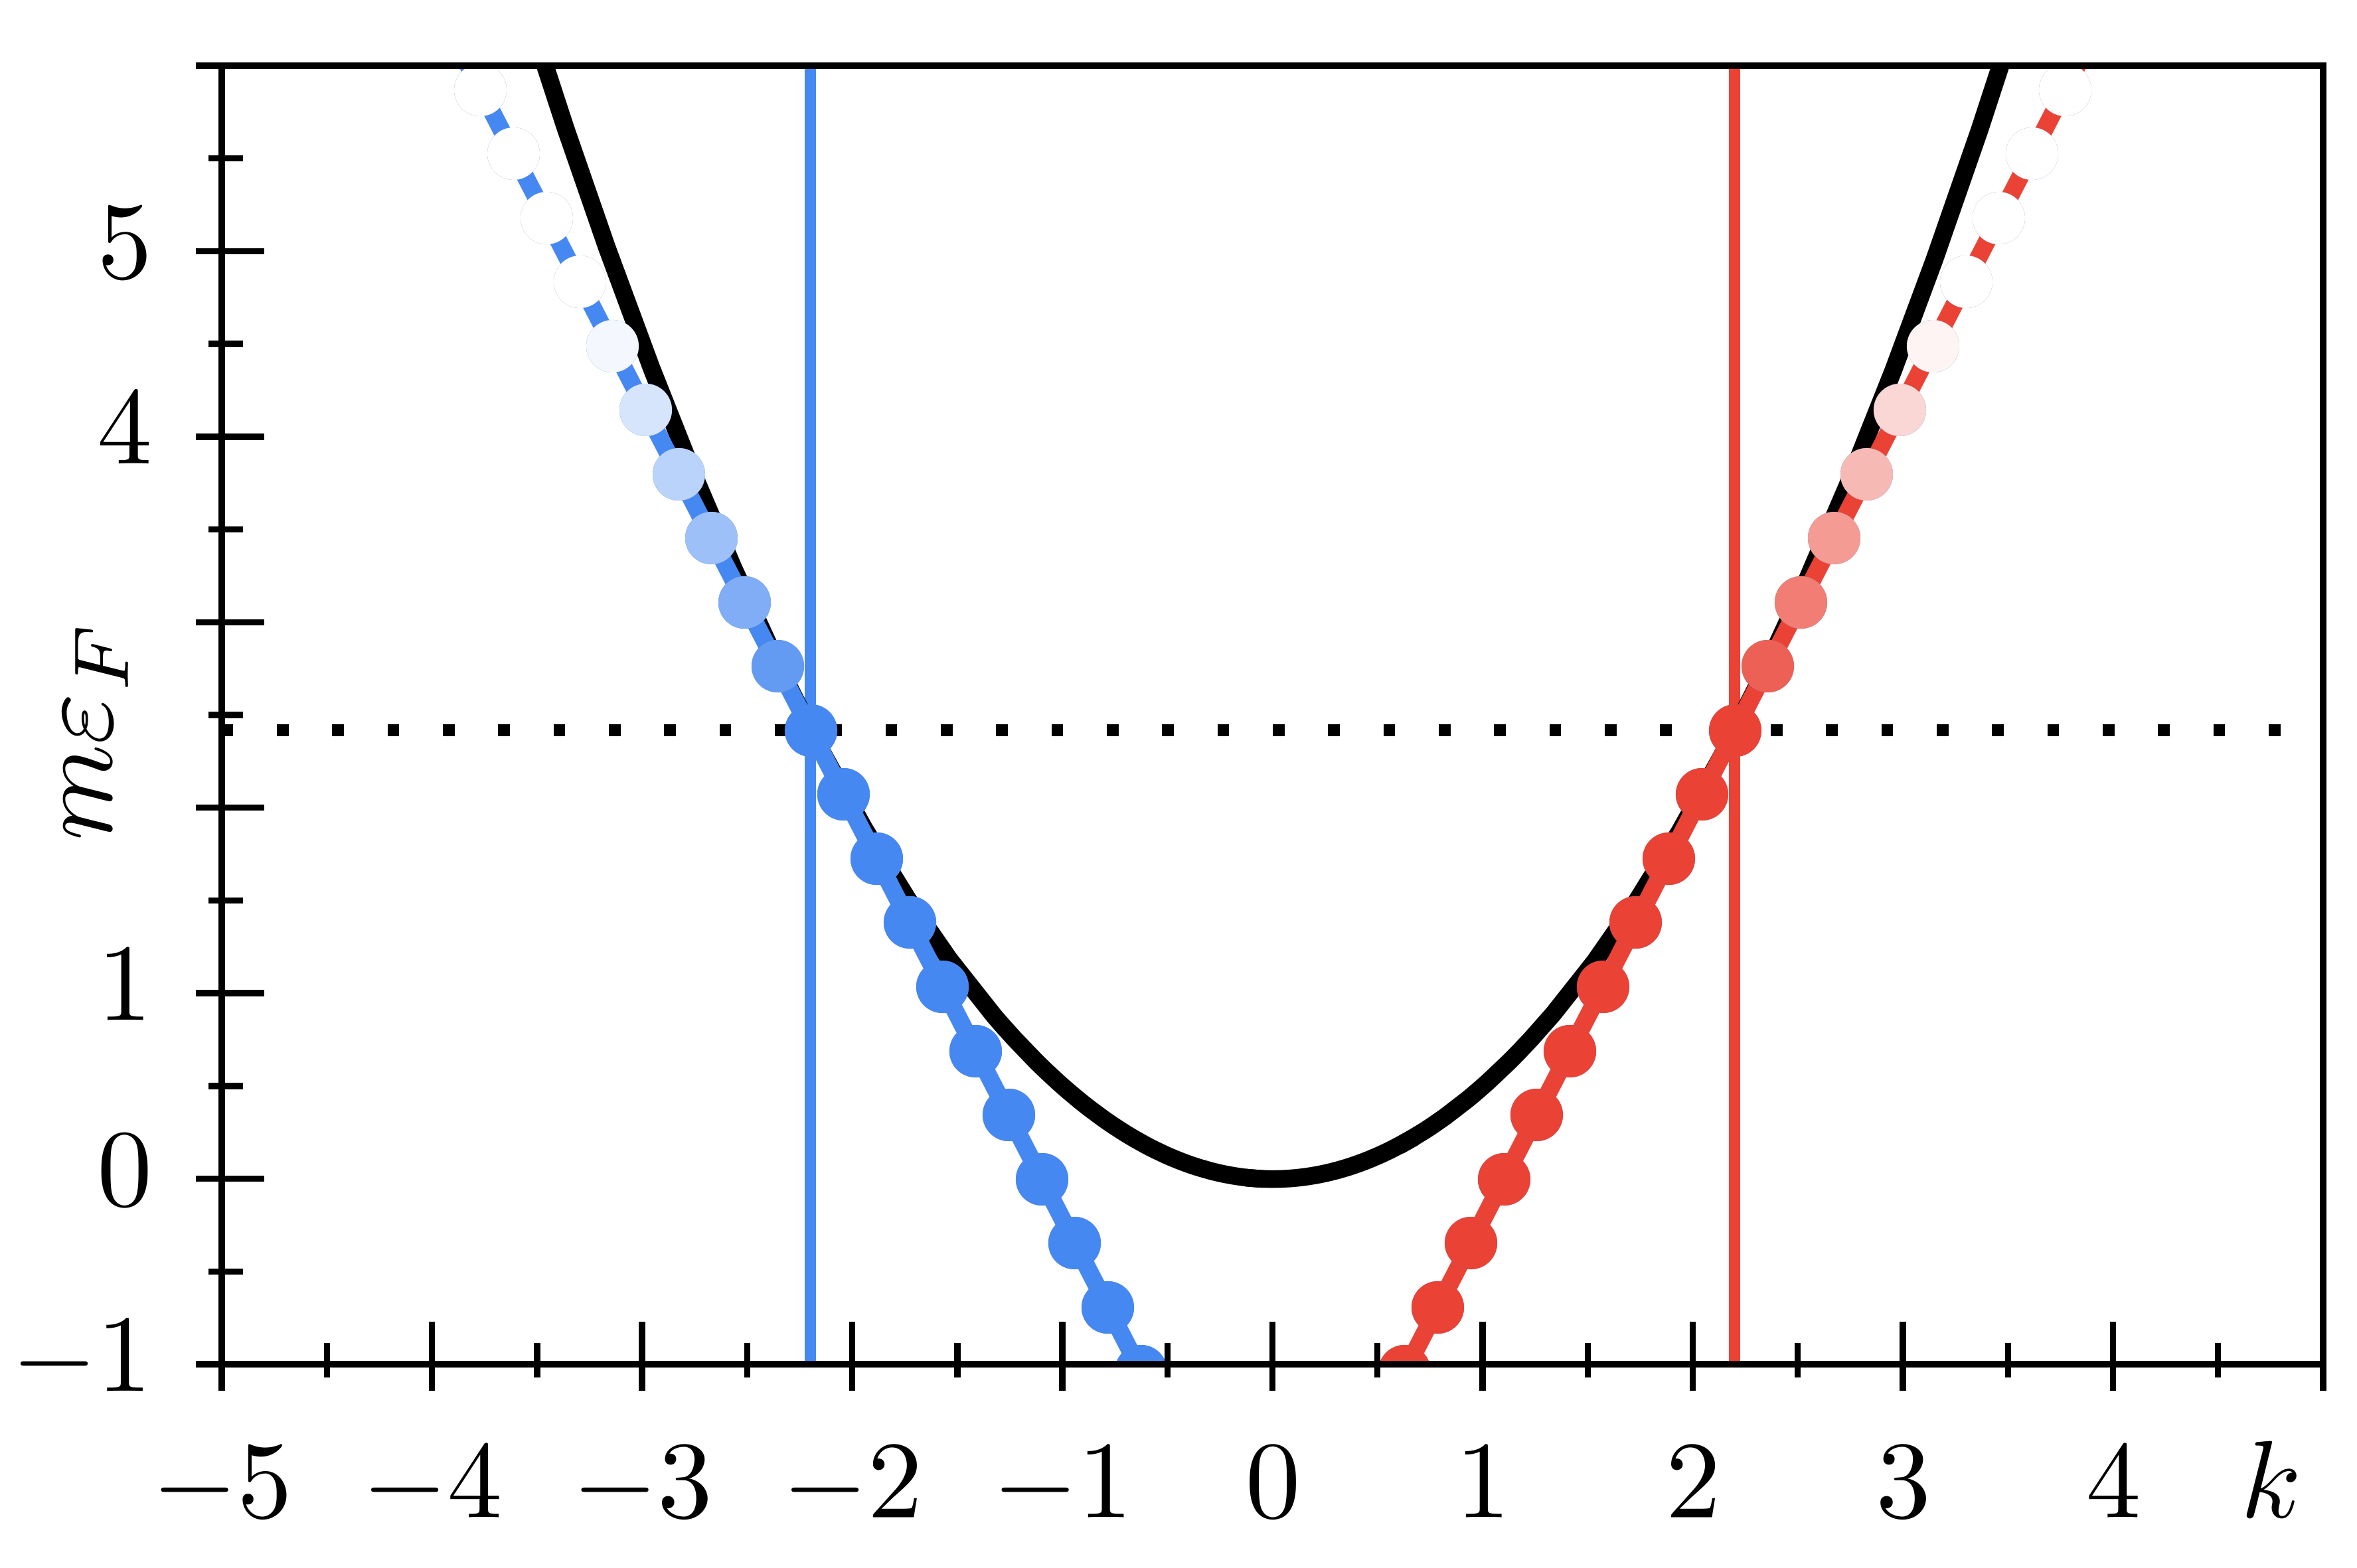
\includegraphics{figures/1D_quadratic_dispersion.png}
    \caption{Quadratic dispersion relation with approximations close to the Fermi energy $\varepsilon_F$.}
    \label{fig:1D_quadratic_dispersion}
\end{figure}
Close to the Fermi energy $\varepsilon_F\coloneqq\varepsilon_{\pm k_F}$, we can approximate the free dispersion and obtain a system of two different species
\begin{align}
    \hat H_0
    &= \sum_k \brlr{\varepsilon_F \pm \frac{k_F}{m}(k\mp k_F) + \mathcal{O}(k^2)}\hat n_k
    \\
    &= \sum_q \brlr{\varepsilon_F + \frac{k_F}{m}q\brlr{\hat n_{q+k_F}-\hat n_{q-k_F}} + \mathcal{O}(k^2)}
    &\approx \sum_{q} v_Fq \brlr{c^\dag_{q,R}c^\pdag_{q,R} - c^\dag_{q,L}c^\pdag_{q,L}}
    \label{eq:dispersion_linearization}
\end{align}
which implies a restriction of $q$ to a small window $|q|<\Gamma\ll m\varepsilon_F$ beyond which \cref{eq:dispersion_linearization} is considered to be invalid.
Note the introduction of the so-called right and left operators $c_{R/L,q}$ which annihilate particles propagating to the left/right with Fermi velocity $\pm v_F=k_F/m$.
\\

For the next part, it will be convenient to understand the meaning of the local density in momentum space, i.e.
\begin{align}
    \hat n(x) = c^\dag_x c^\pdag_x = \frac1L\sum_{k,q}\re^{-\ri x q}c^\dag_{k+q}c^\pdag_{k}.
    \label{eq:local_density}
\end{align}
$\hat n(x)$ thus creates a superposition of particle-hole pairs with characteristic wavelength $q^{-1}$.
The number of particle-hole pairs can be counted through the operator
\begin{align}
    \hat \rho_{-q}\coloneqq \sum_k c^\dag_{k-q}c^\pdag_{k}.
\end{align}
Note further that $\hat\rho_q^\dag = \hat\rho_{-q}$.
By confining the theory close to the Fermi points, there are only two different classes of particle-hole excitations with $q\approx 0$ and $q\approx2k_F$.
The long-wavelength excitations $q\approx0$ are particle-hole pairs of the same species (left or right movers), and excitations of $q\approx2k_F$ are particle-hole pairs of a mixture of the two.
This implies drastic consequences on the relevant action of operators, which we will see in the following.
Let us note here that the density operator of the left/right species $\hat\rho_{\tau,q}$, $\tau\in\{L,R\}$ applied to a Fermi sea creates stable particle-hole excitations (i.e. particles and holes propagate with the same velocity $\pm v_F$) and can thus be used to construct a complete basis of the subspace $\FS^N$ -- for this rather dry discussion, I refer to~\cite{vonDelft1998}.
The consequences of the approximation in \cref{eq:dispersion_linearization} is easily understood in the single-particle operators
\begin{align}
    c^\dag_x = \frac1{\sqrt L}\sum_k \re^{-\ri k x}c^\dag_k \approx \frac1{\sqrt L}\sum_{|q|<\Gamma}\re^{-\ri (q+k_F) x}c^\dag_{R, q} + \re^{-\ri (q-k_F) x}c^\dag_{L, q}
\end{align}
which is then used to find the local density
\begin{align}
    \hat n(x)
    &\approx \frac1L\sum_{q,q'}\brlr{\re^{-\ri (q+k_F) x}c^\dag_{R, q} + \re^{\ri (k_F-q) x}c^\dag_{L, q}}\brlr{\re^{\ri (k_F+q') x}c^\pdag_{R, q'} + \re^{-\ri (k_F-q') x}c^\pdag_{L, q'}},
    \\
    &= \hat \rho_R(x) + \hat \rho_L(x) + \re^{-2\ri k_F}c^\dag_{R}(x)c^\pdag_{L}(x) + \re^{2\ri k_F}c^\dag_{L}(x)c^\pdag_{R}(x).
\end{align}
The first two terms correspond to the $q\approx0$ part of the density, and scattering occurs on the same side of the dispersion relation.
The last two terms scatters right with left movers and transfers particles from one side to the other, which appears at $q\approx2k_F$.
\\

We now turn to an arbitrary two-body interaction of the form~\cref{eq:two_point_interaction} which reads
\begin{align}
    \hat V
    % &= \frac12\int\rd x'\int\rd x V(x'-x)c^\dag(x')c^\dag(x)c^\pdag(x)c^\pdag(x')
    % \\
    &= \frac12\int\rd r\int\rd x V(r)c^\dag(r+x)c^\dag(x)c^\pdag(x)c^\pdag(r+x),
    \\
    &= \frac1{2L^2}\sum_{kk'll'}\int\rd r\int\rd x V(r)\re^{-\ri r(k-l')}\re^{-\ri x(k-l'+k'-l)}c^\dag_kc^\dag_{k'}c^\pdag_lc^\pdag_{l'},
    % \\
    % &= \frac1{2L}\sum_{kk'lq}\int\rd r V(r)\re^{-\ri rq}\delta_{l,k'+q}c^\dag_kc^\dag_{k'}c^\pdag_lc^\pdag_{k-q}
    \\
    &= \frac1{2L}\sum_{kk'q}V(q)c^\dag_kc^\dag_{k'}c^\pdag_{k'+q}c^\pdag_{k-q}
    = \frac1{2L}\sum_{q}V(q)\hat\rho_q\hat\rho^\dag_{q} - \mu.
    \label{eq:two_body_interaction_momentum_space}
\end{align}
The last term is just a constant $\mu = \frac N{2L}\sum_qV(q)$ and can thus be neglected.
By imposing that relevant contributions act close to the Fermi energy involving only momenta in the interval $|k|\in\{k_F\pm\Gamma\}$, we can split the sum in two contributions, one involving scattering processes at small and the other scattering at large momenta
\begin{align}
    \hat V \approx \frac1{2L}\sum_{q\approx0}V(q)\hat\rho_{q}\hat\rho^\dag_{q} + \sum_{q\approx2k_F}V(q)\hat\rho_{q}\hat\rho^\dag_{q}.
\end{align}
For a later study is important to note that the amplitude of the two different $q\approx0$ processes, denoted by $V(q\approx0)$, is equal and independent on the form of the interaction.
A full classification of hypothetical scattering processes is given in~\cref{fig:scattering_processes}.
\begin{figure}
    \centering
    \subfigure[]{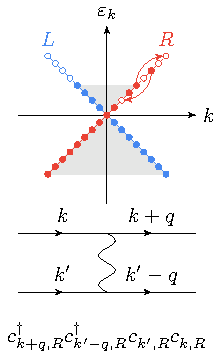
\includegraphics[width=0.328\textwidth]{figures/g4_R.pdf}}
    \subfigure[]{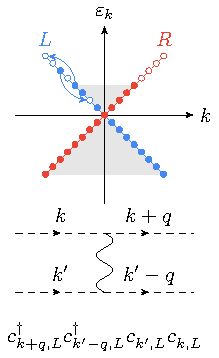
\includegraphics[width=0.328\textwidth]{figures/g4_L.pdf}}
    \subfigure[]{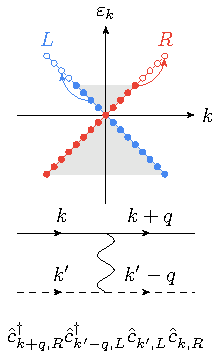
\includegraphics[width=0.328\textwidth]{figures/g2.pdf}}
    \subfigure[]{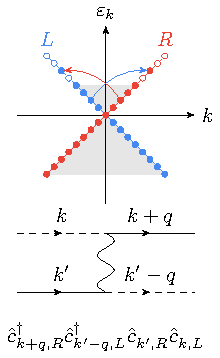
\includegraphics[width=0.328\textwidth]{figures/g1.pdf}}
    \subfigure[]{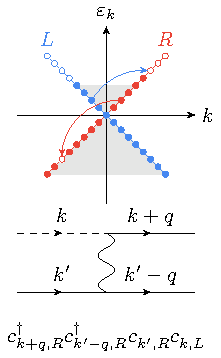
\includegraphics[width=0.328\textwidth]{figures/g13.pdf}}
    \subfigure[]{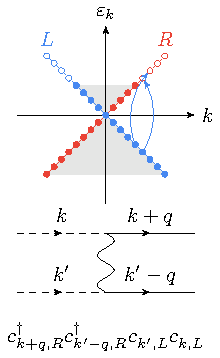
\includegraphics[width=0.328\textwidth]{figures/g22.pdf}}
    \caption{Relevant scattering processes of a generic density-density interaction in one-dimensional quantum systems. (a)/(b) The depicted scattering is commonly referred to as ``forward scattering'' $g_4$ process ($4$ right/left operators, $q\approx0$), (c) as ``backscattering'' $g_2$ process (containing $2$ pairs of right and left operators, $q\approx0$) and (d) as ``Umklapp'' process $g_\perp$ with momentum transfer $q\approx 2k_F$. Other possible scatterings like the ones depicted in (e) and (f) require the existence of high-energy excitations and are thus exponentially suppressed at low temperatures.}
    \label{fig:scattering_processes}
\end{figure}
This simple argumentation allows to consider only the most relevant processes at low temperatures, i.e. those presented in panels (a) - (d).
We will call those processes forward scattering (note that we are discarding chemical potentials on the right hand side of the following equations)
\begin{align}
    g_4\sum_{k,k'}c^\dag_{k+q,\tau}c^\dag_{k'-q,\tau}c^\pdag_{k',\tau}c^\pdag_{k,\tau} = g_4 \hat\rho^\pdag_{q,\tau}\hat\rho^\dag_{q,\tau},
\end{align}
backscattering
\begin{align}
    g_2\sum_{k,k'}c^\dag_{k+q,\tau}c^\dag_{k'-q,\overline\tau}c^\pdag_{k',\overline\tau}c^\pdag_{k,\tau} = g_2 \hat\rho^\pdag_{q,\tau}\hat\rho^\dag_{q,\overline\tau}
\end{align}
and Umklapp scattering
\begin{align}
    g_\perp\sum_{k,k'} c^\dag_{k+q,\tau}c^\dag_{k'-q,\overline\tau}c^\pdag_{k',\tau}c^\pdag_{k,\overline\tau}.
\end{align}
Umklapp terms cannot be expressed in the density operators of the moving modes $\hat\rho_{q,\tau}$ and, for this reason, are discarded here\footnote{Later, we will see that such terms are ``marginal'' and can be neglected under if certain requirements are satisfied (mostly depending on the strength of the interaction $V(q)/t$).}.
Other processes like those depicted in \cref{fig:scattering_processes} (e) and (f) require the existence of high-energy excitations and can thus be neglected for the effective low temperature theory developed here.
In summary, we can express the interaction in terms of the density-density operators as
\begin{align}
    \hat V \approx \frac{1}{2L}\sum_{q,\tau}\brlr{g_4\hat\rho^\pdag_{q,\tau}\hat\rho^\dag_{q,\tau} + g_2\hat\rho^\pdag_{q,\tau}\hat\rho^\dag_{q,\overline\tau}}
    =
    \frac{1}{L}\sum_{q>0}
    \begin{pmatrix}
        \hat\rho^\pdag_{q,R} & \hat\rho^\pdag_{q,L}
    \end{pmatrix}
    \begin{pmatrix}
        g_4 & g_2 \\
        g_2 & g_4
    \end{pmatrix}
    \begin{pmatrix}
        \hat\rho_{-q,R} \\ \hat\rho_{-q,L}
    \end{pmatrix}
    .
    \label{eq:interaction_densities}
\end{align}
\\

To proceed further, it will be useful to compute the commutation of the density operators
\begin{align}
    \commutator{\hat\rho_{q,\tau},\hat\rho_{q',\tau'}}
    =
    \delta_{\tau,\tau'}\sum_k\brlr{c^\dag_{k+q,\tau}c^\pdag_{k-q',\tau}-c^\dag_{k+q+q',\tau}c^\pdag_{k,\tau}}
    \approx
    -\sigma_\tau\delta_{\tau,\tau'}\delta_{q,-q'}\frac{qL}{2\pi}
    \label{eq:chiral_density_commutation}
\end{align}
in which $\sigma_\tau=\pm1$ for $\tau=R/L$, respectively, and the right hand side is obtained through a projection on the ground state\footnote{This is a reasonable approximation for small interactions only (as a result from a first order perturbative expansion). For a more thorough discussion of \cref{eq:chiral_density_commutation}, see~\cite{Giamarchi2003}.}.
We are now in shape to define canonical bosonic operators representing the interaction degrees of freedom for $q>0$
\begin{align}
    b^\dag_{+q} \coloneqq \sqrt\frac{2\pi}{qL}\hat\rho_{-q,L},
    \quad
    b^\pdag_{+q} \coloneqq \sqrt\frac{2\pi}{qL}\hat\rho_{+q,L},
    \\
    b^\dag_{-q} \coloneqq \sqrt\frac{2\pi}{qL}\hat\rho_{+q,R},
    \quad
    b^\pdag_{-q} \coloneqq \sqrt\frac{2\pi}{qL}\hat\rho_{-q,R},
    \label{eq:canonical_bosonic_operators}
\end{align}
that satisfy the commutation relation $\commutator{b_q^\pdag,b_{q'}^\dag} = \delta_{q,q'}$.
Using \cref{eq:canonical_bosonic_operators} results in a familiar expression for the interaction written in \cref{eq:interaction_densities}, i.e.
\begin{align}
    \hat V \approx\sum_{q>0}\frac{q}{2\pi}
    \begin{pmatrix}
        b_q & b^\dag_{-q}
    \end{pmatrix}
    \begin{pmatrix}
        g_4 & g_2 \\
        g_2 & g_4
    \end{pmatrix}
    \begin{pmatrix}
        b^\dag_q \\ b_{-q}
    \end{pmatrix}
    .
    \label{eq:quadratic_interactions}
\end{align}
The interaction, originally quartic in the fermionic degrees of freedom, can be cast into a (quadratic) sum of bosonic operators which are the low-energy excitations of the original model.
All that is left to do is to cast the kinetic term into this new basis, which is actually a quite lengthy calculation if we were to approach it by brute-force.
There is an indirect reasoning through Schur's lemma: if two operators $\hat H$ and $\hat H'$ have identical commutation relations with all $\{c^\pdag_\alpha,c^\dag_\alpha\}$, then the two operators are equal up to a chemical potential.
One can easily verify the commutator of the mover-density with the kinetic Hamiltonian
\begin{align}
    \commutator{\hat H_0, \hat\rho_{q,\tau}}
    =
    \sum_{p,\tau'}v_F\sigma_{\tau'}\commutator{\hat n_{p,\tau'},\hat\rho_{q,\tau}}
    =
    \sigma_\tau v_F q \hat\rho_{q,\tau}
\end{align}
and find its equivalent expression in bosonic degrees of freedom to be
\begin{align}
    \hat H_0' = \frac{\pi v_F}L\sum_{q,\tau}\hat\rho_{q,\tau}\hat\rho_{-q,\tau} = \frac{2\pi v_F}L\sum_{q>0,\tau}\hat\rho_{q,\tau}\hat\rho_{-q,\tau},
\end{align}
which can be verified through evaluation of
\begin{align}
    \commutator{\hat H_0',\hat\rho_{q,\tau}}
    \overset{\text{\cref{eq:recursive_commutation}}}{=}
    -\frac{\pi v_F}L
    \sum_{p,\tau'}
    \brlr{
    \commutator{\hat\rho_{q,\tau},\hat\rho_{p,\tau'}}\hat\rho_{-p,\tau'}
    -
    \hat\rho_{p,\tau'}\commutator{\hat\rho_{q,\tau},\hat\rho_{-p,\tau'}}
    }
    =
    \sigma_\tau v_F q\hat\rho_{q,\tau}
\end{align}
and thus we conclude our previous statement $\hat H_0' = \hat H_0 + \mu$ with an irrelevant constant $\mu$.
The effective low energy Hamiltonian containing kinetic and interaction energy satisfies the following matrix equation
\begin{align}
    \hat H = \hat H_0 + \hat V \approx
    \sum_{q>0}\frac{q}{2\pi}
    \begin{pmatrix}
        b_q & b^\dag_{-q}
    \end{pmatrix}
    \begin{pmatrix}
        2\pi v_F + g_4 & g_2 \\
        g_2 & 2\pi v_F + g_4
    \end{pmatrix}
    \begin{pmatrix}
        b^\dag_q \\ b_{-q}
    \end{pmatrix}
    .
    \label{eq:luttinger_hamiltonian_nondiagonal}
\end{align}
As a final step, we want to find the spectrum of the previous Hamiltonian through a basis transformation $B_q = T B'_q$\footnote{The matrix coupling the dot product of the operator spinors $B_q$ is independent on the momentum $q$ and as such the basis transformation $T$ will not depend on $q$ as well.} with $B_q = (b_q^\dag, b_{-q})^T$ such that
\begin{align}
    \hat H = \sum_{q>0} qB^\dag_q H B^\pdag_q = \sum_{q>0} qB'^\dag_q T^\dag H T B'^\pdag_q
\end{align}
is in its diagonal form.
Naive (unitary) rotations do not preserve the commutators of the spinor $B$, defined through
\begin{align}
    \commutator{B_{q,i}^\pdag,B^\dag_{q,j}} = \commutator{B_{q,i}'^\pdag,B'^\dag_{q,j}} = (-\sigma_z)_{i,j}
\end{align}
which imposes an additional constraint on the transformation $T$ according to
\begin{align}
    T^\dag\sigma_z T = \sigma_z,
    \quad
    T^\dag = \sigma_zT^{-1}\sigma_z.
\end{align}
We thus find the similarity relation between the original and the rotated basis according to
\begin{align}
    H'=T^\dag HT =\sigma_z T^{-1}\sigma_z H T,
\end{align}
which allows us to solve the eigenvalue equation of $\sigma_z H$ without knowing the explicit form of $T$.
Since $\sigma_zH$ has vanishing trace, its spectrum is symmetric $\pm E$ and we arrive at the appealing result $H' = E\mathbb1$ with the $2\times2$ unit matrix $\mathbb1$ and scalar eigenvalue
\begin{align}
    E = \frac1{2\pi}\sqrt{\brlr{2\pi v_F + g_4}^2 - g_2^2}
\end{align}
leading to the identity
\begin{align}
    \hat H' = \sum_{q>0} Eq B'^\dag_q B'^\pdag_q = \sum_{q>0} \omega_q B'^\dag_q B'^\pdag_q.
\end{align}
Notice that we succeeded to rewrite the original problem to a sum of decoupled Harmonic oscillators with frequencies $\omega_q\coloneqq Eq$.
%
%
%%%%%%%%%%%%%%%%%%%%%%%%%%%%%%%%%%%%
\section{The harmonic oscillator}
\label{sec:the_harmonic_oscillator}
%%%%%%%%%%%%%%%%%%%%%%%%%%%%%%%%%%%%
% %
% %
% %%%%%%%%%%%%%%%%%%%%%%%%%%%%%%%%%
% %%%%%%%%%%%%%%%%%%%%%%%%%%%%%%%%%
% \section{Matrix product states}
% \label{sec:matrix_product_states}
% %%%%%%%%%%%%%%%%%%%%%%%%%%%%%%%%%
% %%%%%%%%%%%%%%%%%%%%%%%%%%%%%%%%%
% %
% %
% %%%%%%%%%%%%%%%%%%%%%%%%%%%%%%%%%%
% \subsection{Exact diagonalization}
% \label{sec:exact_diagonalization}
% %%%%%%%%%%%%%%%%%%%%%%%%%%%%%%%%%%
% %
% %
% %%%%%%%%%%%%%%%%%%%%%%%%%%%%%%%%%%
% \subsection{Schmidt decomposition}
% \label{sec:schmidt_decomposition}
% %%%%%%%%%%%%%%%%%%%%%%%%%%%%%%%%%%
% %
% %
% %%%%%%%%%%%%%%%%%%%%%%%%%%%%%%%%%%%%%%%%%%%%
% \subsection{Variational ground state search}
% \label{sec:variational_ground_state_search}
% %%%%%%%%%%%%%%%%%%%%%%%%%%%%%%%%%%%%%%%%%%%%
% %
% %
% %%%%%%%%%%%%%%%%%%%%%%%%%%%
% \subsection{Time evolution}
% \label{sec:time_evolution}
% %%%%%%%%%%%%%%%%%%%%%%%%%%%
% %
% %
% %%%%%%%%%%%%%%%%%%%%%%%%%%%%%%%%%%%%%%%%
% %%%%%%%%%%%%%%%%%%%%%%%%%%%%%%%%%%%%%%%%
% \section{Topological phases of matter}
% \label{sec:topological_phases_of_matter}
% %%%%%%%%%%%%%%%%%%%%%%%%%%%%%%%%%%%%%%%%
% %%%%%%%%%%%%%%%%%%%%%%%%%%%%%%%%%%%%%%%%
% %
% %
% %%%%%%%%%%%%%%%%%%%%%%%%%%%%%%%%%%%%%%%%%%%
% \subsection{The Su-Schrieffer-Heeger chain}
% \label{sec:the_ssh_chain}
% %%%%%%%%%%%%%%%%%%%%%%%%%%%%%%%%%%%%%%%%%%%
% %
% %
% %%%%%%%%%%%%%%%%%%%%%%%%%%%%%%%%%%%%%%%%%%%%%%%%%%%%%%%%%%
% \subsection{Symmetry classification of topological phases}
% \label{sec:symmetry_classification_of_topological_phases}
% %%%%%%%%%%%%%%%%%%%%%%%%%%%%%%%%%%%%%%%%%%%%%%%%%%%%%%%%%%
%
%
%%%%%%%%%%%%%%%%%%%%%%%%%%%%%%%%%%%%%%%%%%%%%%%%%%%%%%%
%%%%%%%%%%%%%%%%%%%%%%%%%%%%%%%%%%%%%%%%%%%%%%%%%%%%%%%
\chapter{Ultracold atoms trapped in optical lattices}
\label{ch:ultracold_atoms_trapped_in_optical_lattices}
%%%%%%%%%%%%%%%%%%%%%%%%%%%%%%%%%%%%%%%%%%%%%%%%%%%%%%%
%%%%%%%%%%%%%%%%%%%%%%%%%%%%%%%%%%%%%%%%%%%%%%%%%%%%%%%
